\subsection{Rational Trust Assumptions}%
\label{sub:probabilistic_trust}
In our approach to a randomness beacon we want to push beyond the need for honest operators and naïve users.
To achieve this we extend the work of \citet{randomzoo} to quantify trusting the beacon and then determine thresholds for reasonable behavior when using delay functions.
This effectively provides a measure of rational trust, where users decide for themselves if what they have observed is adequate.

We present a property which, if satisfied, means a user can trust that the beacon operator is not capable of fooling them.
This property is true if the user determines that nobody is able to compute the delay function in the time between the users input and the user receiving the beacon's commitment.
This can be condensed to:
\begin{equation*}
    t_\text{COMMITMENT} - t_\text{INPUT}\enspace <\enspace T_\text{DELAY FUNCTION}
\end{equation*}
given that $t_\text{INPUT}$ is the time when the user sent the input, $t_\text{COMMITMENT}$ is when the user received the commitment, and $T_\text{DELAY FUNCTION}$ is the fastest computation of the delay function.
So for users to be more likely to trust a beacon, the time between sending the input and receiving the commitment must be significantly smaller than the time between the commitment and the output.
In fact, it must be smaller than the shortest time the user thinks the operator could compute the delay function.

An example could be that a user believes that the world's fastest computer can compute the delay function in 2 minutes.
In this case the user can trust the output if he sees a commit to a set of inputs containing his input within 2 minutes of his input, because then he knows that nobody could have had time to run the computation on his input before choosing to release a commitment or not.
This relation between the time taken to compute the delay function and the time before a commit is seen allows users to flexibly adjust their willingness to trust the outcome has not been biased against them.

This threshold is also described by \citet{randomzoo}, where they advise a ratio of no more than $\frac{1}{5}$ of the computation time spent collecting inputs.
In their paper, \citeauthor{randomzoo} furthermore state that smart participants will always try to minimize the time between their input and the commitment.
We see this as potentially problematic, since such behavior can create congestion in the system, which might result in some inputs not being used in the intended output computation.
This means that users whose inputs were not included cannot trust the output of the given beacon iteration.

Taking all this into consideration we present a beacon operation protocol which can be adjusted to increase or decrease the ratio and thereby the limit for probabilistic trust.
The operation must be sequential which means that we must collect input before computing the delay function.
However, because we want to spend more time computing than we are collecting input, a strictly sequential beacon will contain dead spots where no user is submitting input.
This may be acceptable in some scenarios, but we want to design a beacon which always accepts inputs and will not be suspected of malicious operation.
To achieve this we parallelize the beacon protocol, meaning that several delay functions run in parallel but offset in time and on different input.
In \cref{fig:beacon_parallel_timeline} this is illustrated, where these offset but parallel beacons are seen.

\begin{figure}[htb]
    \centering
    \footnotesize
    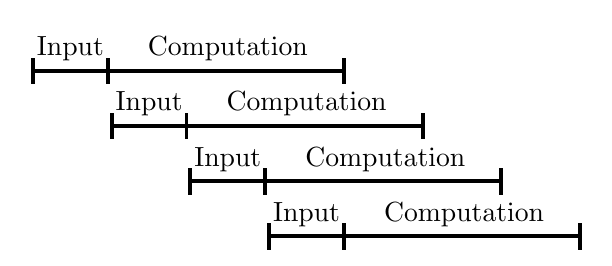
\begin{tikzpicture}
    \foreach \x in {0, ..., 3} {
        \draw[|-|, black, line width=0.5mm] (\x,-\x*0.7) to (\x+1,-\x*0.7);
        \path (\x,-\x*0.7) -- (\x+1,-\x*0.7) node [midway, above] {Input};
        \draw[-|, black, line width=0.5mm, shorten <=-0.1mm] (\x+1,-\x*0.7) to (\x+4,-\x*0.7);
        \path (\x+1,-\x*0.7) -- (\x+4,-\x*0.7) node [midway, above] {Computation};
    }
    \end{tikzpicture}
    \caption{Parallelized beacon protocol, with offset input collection and overlapping computation.
After every computation the output is published.}\label{fig:beacon_parallel_timeline}
\end{figure}

We observe that no input collection is run in parallel nor overlapping, which resembles a constant stream of input collection.
In addition, the computation components can eventually be reused for future beacon computations, thereby eliminating the need for spinning up new computation services.
These observations are depicted in \cref{fig:beacon_parallel_timeline_real}, where the beacon would output at each circle shown in the diagram.

\subimport{}{timeline_diagrams.tex}

\subsubsection{Number of Computation Nodes}
The number of computation nodes required in this fashion is the duration of the delay function divided by the duration of input collection:
\begin{equation*}
    \text{Number of Nodes} = \left\lceil\frac{T_\text{DELAY FUNCTION}}{T_\text{INPUT COLLECTION}}\right\rceil
\end{equation*}

\noindent
As an example, an input collection time of 2 minutes and a delay function of 10 minutes will require 5 computation nodes to always begin a computation every 2 minutes.

However, the delay function is not guaranteed to precisely take e.g.\ 10 minutes --- the computation nodes are expected to be running other processes such as an operating system which also require some CPU time.
Therefore, the delay function can be expected to from time to time finish a bit later than naïvely anticipated.
This will over time cause the beacon output to be increasingly more skewed compared to the initial output frequency, since they can only be delayed and not catch up by being faster sometimes.

To remedy this, a number of additional nodes should be kept at hand.
Therefore, we update the prior equation to take this extra time for each delay function into account.
Let $\delta$ be this extra time additional to the delay function.
\begin{equation*}
    \text{Number of Nodes} = \left\lceil\frac{T_\text{DELAY FUNCTION}+\delta}{T_\text{INPUT COLLECTION}}\right\rceil
\end{equation*}

\noindent
If, for example, the delay function is expected to always finish at most 2 minutes later than the expected time of 10 minutes (i.e.\ a worst-case time of 12 minutes) and the input collection is 2 minutes, 6 nodes in total are necessary to guarantee a node is always ready every 2 minutes, given a maximum of 2 minutes expected delay.

The beacon operator should find a sensible number of nodes that maximizes the chances of a ready computation node given expected delays, while minimizing the idle time of the nodes.

\subsubsection{Expected User Behavior}
Based on what \citet{randomzoo} write about smart users always trying to input as close to the commitment as possible, we admit that our solution of parallel offset computations will not prevent such behavior.
However, the goal of our approach is not to eliminate this user strategy, but to minimize the need for it.

In our beacon we do not expect to give guarantees about deadlines, such as commitment and output publishing, since such guarantees only would serve as false reassurance to the user.
Instead, our beacon is adjustable, such that a ratio of input collection and computation time, which most users finds reasonable, can be deployed.

Users are still welcome to contribute input as close to a deadline as possible in order to gain a better probabilistic guarantee.
This may, however, be tricky as the beacon will not announce deadlines as to not encourage users to input at the same time.
Instead, we propose another strategy for the smart user: Instead of supplying one input, multiple unique inputs should be supplied spaced apart in time.
For example, a user supplying an input every 10 seconds until receiving a commitment will have a better chance of coming close to the deadline.
